\documentclass[12pt, oneside]{article}
\usepackage[hidelinks]{hyperref}
\usepackage[T1]{fontenc}
\usepackage{amssymb, amsmath, amsthm, mathtools, systeme, parskip, graphicx, multirow, xifthen}
\usepackage[margin=1cm, a5paper, top=20mm, headheight=110pt, voffset=0pt, footskip=14.5pt]{geometry}
\renewcommand{\familydefault}{\sfdefault}
\setlength{\jot}{15pt}

\makeatother
\def\@lecture{}%
\newcommand{\lecture}[3]{
    \ifthenelse{\isempty{#3}}{%
        \def\@lecture{Lecture #1}%
    }{%
        \def\@lecture{Lecture #1: #3}%
    }%
    \subsection{\@lecture}
    \def\date{#2}%
}
\makeatletter

\makeatother
\usepackage{fancyhdr}
\pagestyle{fancy}

\fancyhead[L]{\@lecture}
\fancyhead[R]{\date}

\fancyfoot[L]{\thepage}  % Right odd,  Left even
\fancyfoot[R]{}          % Right even, Left odd
\fancyfoot[C]{\rightmark}     % Center

\makeatletter
\usepackage[swedish]{babel}

\title{Matematik 2B \\ Sammanfattning}
\author{Otto Martinwall}

\begin{document}
\maketitle
\tableofcontents
\newpage

\newtheorem{definition}{Definition}
\newtheorem{theorem}{Theorem}

\section{Förkunskaper (träna detta så att det sitter!)}
\subsection{Negativa tal}

Ett negativt tal är bara den additiva inversen av samma tal. Om $a$ är ett reellt tal och $-a$ är dess additiva invers, så är $a+(-a)=0$. Ett sätt att se på det är att den additiva inversen (negativa varianten) av ett tal är lika långt från $0$ på tallinjen, men åt andra hållet. 

Multiplikation får några egenskaper utav detta, som att negativt gånger negativt blir positivt. Att vända dig om och sedan backa blir detsamma som att bara gå rakt fram från början.

Några regler kring detta är då:

\begin{align}
	(-a)(-b) = ab \\
	(-a)b = -ab \\
	a(-b) = (-a)b \\
	\frac{(-a)}{b} = \frac{a}{(-b)}
\end{align}

\newpage
\subsection{Prioriteringsregler}

Prioriteringsregler har vi, då att om vi fick välja helt fritt så skulle alla få olika svar. Ordningen är såhär:

\begin{enumerate}
	\item Paranteser
	\item Multiplikation/Division 	
	\item Addition/Subtraktion
\end{enumerate}

Om två av samma prioritet är efter varann, börja från vänster.

Ett exempel är 

\begin{align*}
	6\div 2(1+2) = \\
	6\div 2(3) = \\
	6\div 2 \cdot 3 = \\
	3 \cdot 3 = \\
	9
\end{align*}

\newpage
\subsection{Bråk}

Bråk är tal som representeras som kan skrivas som en kvot\footnote{resultatet av en division} av två heltal. Det kan t.ex vara $\frac{3}{7}$, vilket kan tänkas som  \textit{tre sjundedelar}.

\subsubsection{Addition av bråk}
\label{Addition av bråk}
Lättaste metoden för addition av bråk är att skriva om bråken så att de får samma nämnare\footnote{nedre parten hos ett bråk}:

\begin{align}
	\frac{1}{3} + \frac{3}{4} = \\
	\frac{1\cdot 4}{3\cdot 4} + \frac{3\cdot 3}{4\cdot 3} = \\
	\frac{4}{12} + \frac{9}{12} = \\
	\frac{13}{12}
\end{align}

Metoden jag brukar använda för att skriva om bråken, är att multiplicera täljaren och nämnaren på det ena bråket, med nämnaren på det andra, och tvärt om. I exemplet ovan så har ena bråket nämnaren 3, så jag multiplicerar täljaren och nämnaren med just 3 på det andra bråket, och tvärt om med talet 4 på det förstnämnda bråket. Genom denna metod får bråken samma nämnare då $ab = ba$, som ses i nämnarna på rad (6) till (7). Efter det så kan man addera täljarna på bråken.

Addition och subtraktion fungerar likadant här.

\subsubsection{Multiplikation av bråk}

Multiplikation av bråk är mycket enkelt.

\begin{align}
	\frac{a}{b} \cdot \frac{c}{d} = \frac{ac}{bd}
\end{align}

\subsubsection{Division av bråk}
\label{Division av bråk}

Division är en typ av multiplikation, vilket gör denna ganska enkel men aningen klurigare. Division är inversen av multiplikation, så att dividera med $5$ är samma sak som att multiplicera med $\frac{1}{5}$. Detta resulterar i att:

\begin{align}
	\frac{a}{b} \div\frac{c}{d} = \\ 
	\frac{a}{b} \cdot \frac{d}{c} = \\
	\frac{ad}{bc}
\end{align}

Det andra bråket vänder alltså bara på sig vid utbytet av divisionstecken mot multiplikationstecken.

\newpage
\subsection{Potenser}
\label{Potenser}

Potenser kan ses som repeterad multiplikation i vissa fall\footnote{andra definitioner krävs för att inkludera alla reella eller till och med komplexa exponenter. Det kommer först i universitetsmatten.}. Alltså att om exponenten\footnote{En exponent är den övre delen av en potens, alltså det som brukar komma efter man säger \textit{upphöjt till}} $n$ är ett positivt heltal så gäller detta:

\begin{align}
	a^n = a_1 \cdot a_2 \cdot ... \cdot a_n
\end{align}

\textit{Roten ur} kan skrivas på två sätt, där $n$ är ett positivt heltal:

\begin{align}
	\sqrt[n]{a} = a^{\frac{1}{n}}
\end{align}

\newpage
\subsubsection{Potensregler}


Dessa regler gäller för alla tal, alltså inte bara heltal för exponenterna.

\begin{align}
	a^ba^c = a^{b+c} \\
	\frac{a^b}{a^c} = a^{b-c} \\
	(a^b)^c=a^{bc} \\
	(ab)^x=a^xb^x \\
	\left(\frac{a}{b}\right)^x=\frac{a^x}{b^x} \\
	a^{-b} = \frac{1}{a^b} \\
	a^0 = 1
\end{align}

\newpage
\subsection{Ekvationer}

En ekvation är ett typ av påstående, som innehåller en eller fler variabler (okända). Jag kan påstå att $3x+2 = 8$ utan att säga vad $x$ är. Just detta är endast sant om $x=2$.

Ekvationer brukar kräva att man löser ut enskilda variabler i slutändan. Metoden jag brukar ha är att först och efter varje steg se om jag kan förenkla ekvationen genom addition/subtraktion, sedan om det går genom multiplikation/division, och till sist om det går genom potenser.

\paragraph{Exempel 1}

\begin{align}
	\frac{x}{x+10} = \frac{24}{54}
\end{align}

Först så letar jag om jag kan göra något med addition/subtraktion, vilket inte hjälper här. Nästa möjlighet är om multiplikation/division kan förenkla något, vilket det kan genom multiplikation av $x+10$ på båda sidor\footnote{Detta förenklar då multiplikation är lättare att hantera än division, så vi vill få bort divisionstecken.}

\begin{align}
	x = \frac{24}{54}(x+10)
\end{align}

Nu kollar vi igen. Addition/subtraktion hjälper inget, men multiplikation/division hjälper återigen här. Vi förenklar genom att multiplicera in i parantesen.

\begin{align}
	x = \frac{24}{54}x + \frac{24}{54} \cdot 10
\end{align}

Återigen så letar vi. Addition/subtraktion verkar hjälpa denna gång då målet är att få x på samma sida av likhetstecknet. Vi subtraherar med $\frac{24}{54}x$. I samma veva kan vi även multiplicera in $10$ i bråket på höger sida.

\begin{align}
	x - \frac{24}{54}x = \frac{24}{54} \times 10 \\
	x - \frac{24}{54}x = \frac{240}{54}
\end{align}

Nu så kikar vi igen. Multiplikation/divison hjälper för att möjliggöra subtraktion av bråken på vänster sida av likhetstecknet, genom att låta dem få samma nämnare som i \ref{Addition av bråk}.

\begin{align}
	\frac{54}{54}x - \frac{24}{54}x = \frac{240}{54}
\end{align}

Nu kan vi alltså subtrahera bråken på vänster sida väldigt lätt.

\begin{align}
	\frac{30}{54}x = \frac{240}{54}
\end{align}

Här så hjälper inte addition/subtraktion, men multiplikation/division gör. Vi dividerar med $\frac{30}{54}$ för att $x$ ska bli ensam på vänsterledet.

\begin{align}
	x = \frac{240}{54} \div \frac{30}{54}
\end{align}

Här så kan vi ändra om från division av bråken till multiplikation av bråken, på sättet beskrivet i \ref{Division av bråk}.

\begin{align}
	x = \frac{240}{54} \times \frac{54}{30}
\end{align}

$54$ i nämnaren på första bråket och i täljaren på andra bråket tar ut varann, och resterande steg bör gå rätt smidigt:

\begin{align}
	x = \frac{240}{30} \\
	x = \frac{24}{3} \\
	x = 8
\end{align}

\paragraph{Exempel 2}

\begin{align}
	x^{\frac{1}{3}} = 3
\end{align}

Här så fungerar inte addition/subtraktion, eller multiplikation/division. Nästa sak att checka är alltså potenser. Här så kan vi använda oss av potensreglerna i \ref{Potenser}, där $(a^b)^c = a^{bc}$, för att ändra exponenten hos $x$ från $\frac{1}{3}$ till $1$.

\begin{align}
	(x^{\frac{1}{3}})^{3} = (3)^3 \\
	x^{\frac{3}{3}} = 27 \\
	x^1 = 27 \\
	x = 27
\end{align}

\newpage
\subsection{Pythagoras Sats}
\label{Pythagoras Sats}

Denna är kort, men viktig. 

\begin{theorem}
	För en rätvinklig triangel med sidlängderna $a$ och $b$ för vardera katet\footnote{de kanter som är direkt anslutna med det rätvinkliga hörnet} och $c$ för hypotenusan, så gäller det att 

	\begin{align}
		a^2+b^2=c^2
	\end{align}
\end{theorem}

\newpage
\subsection{Inversfunktion (viktigt till logaritmer)}
\label{Inversfunktion}

En inversfunktion är en funktion som gör exakt motsatt av originalfunktionen. Om $g(x)$ är inversfunktionen till $f(x)$, och $f(x)$ mappar\footnote{med mappar så menar jag att om jag sätter in värdet $1$ i funktionen, alltså att $x=1$, så ger funktionen $f(x)$ ut något värde beroende på värdet jag satte in, och om det är $3$ så mappar $f(x)$ $1 \rightarrow 3$.} $a \rightarrow b$, så mappar $g(x)$ $b \rightarrow a$.

På grund av detta så kan man grafiskt se att en inversfunktion speglas runt linjen y=x till originalfunktionen. En annan konsekvens är att $f(g(x))=x$ då $g(x)$ bara mappar tillbaka igen till det ursprungliga värdet.

\subsubsection{Exempel}

Vi väljer att $f(x) = 2x + 2$. Vi låter $g(x)$ vara inversfunktionen av $f(x)$. Då $f(x)$ är en linjär funktion så kommer inversen av $g(x)$ också vara linjär då $g(x)$ är spegelbilden av $f(x)$ runt linjen $y=x$. Därmed kan vi konstatera att
\begin{align}
	g(x)=kx+m.
\end{align}
För att ta reda på $k$ och $m$ så kan vi skapa ett ekvationssystem med hjälp av att vi vet att $g(x)$ är inversen av $f(x)$.
\begin{align}
	f(0) = 2 \Rightarrow g(2) = 0 \\
	f(1)=4 \Rightarrow g(4)=1
\end{align}
Jag väljer att använda additionsmetoden från \ref{Additionsmetoden}.
\begin{align}
	\begin{cases}
		2k+m = 0 \\
		4k+m = 1
	\end{cases}
\end{align}
\begin{align}
	\begin{cases}
		-2k-m = 0 \\
		4k+m = 1
	\end{cases}
\end{align}
\begin{align}
	\begin{cases}
		-2k-m = 0 \\
		2k = 1
	\end{cases}
\end{align}
\begin{align}
	\begin{cases}
		-2k-m = 0 \\
		k = \frac{1}{2}
	\end{cases}
\end{align}
\begin{align}
	\begin{cases}
		-m = 1 \\
		k = \frac{1}{2}
	\end{cases}
\end{align}
\begin{align}
	\begin{cases}
		m = -1 \\
		k = \frac{1}{2}
	\end{cases}
\end{align}

Detta betyder då att

\begin{align}
	g(x) = \frac{1}{2}x-1.
\end{align}

Om vi nu tittar på $f(x)$ och $g(x)$ grafiskt så ser det ut såhär:

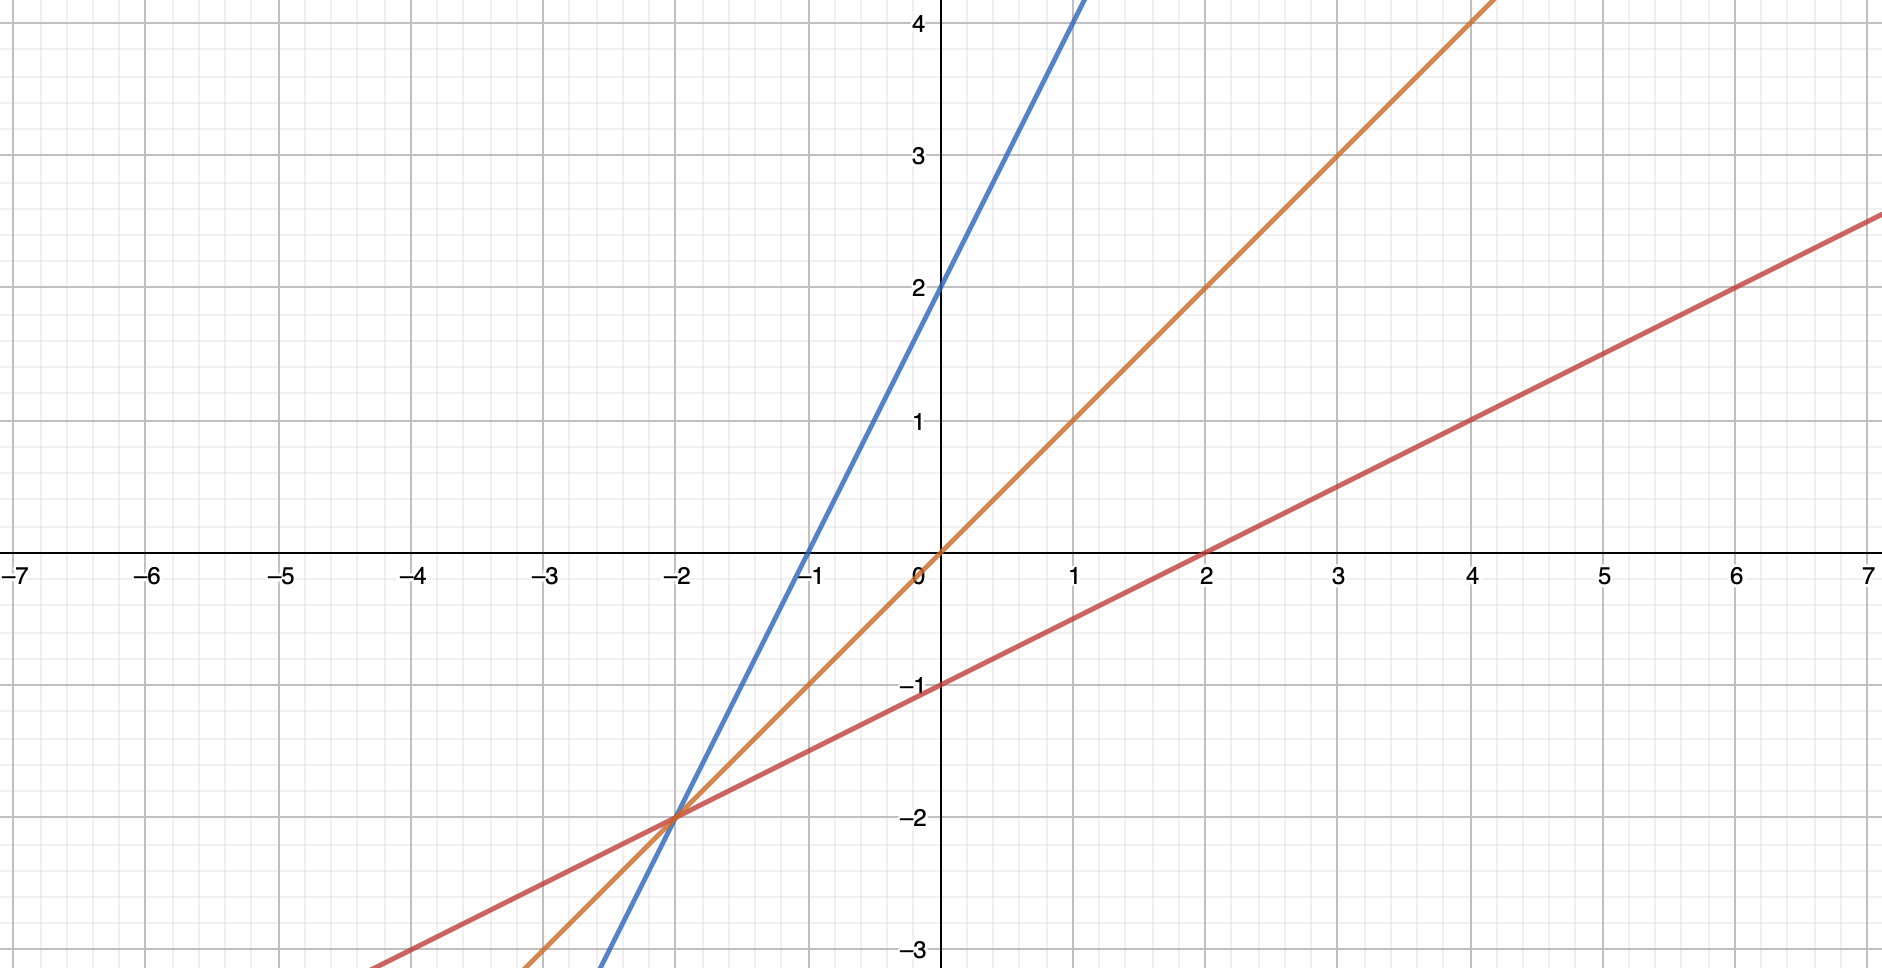
\includegraphics[width=\textwidth]{img/5.png}

I bilden är $f(x)$ den blåa linjen och $g(x)$ är den röda. Linjen som de speglas runt är $y=x$ som är orange här.

Vi kan se i bilden att t.ex så är $f(1)=4$ och att om vi då stoppar in det värde $f(x)$ kastade ut, in i $g(x)$, så får vi $g(4)=1$ vilket gör att vi bara får tillbaka det värde vi hade innan. $g(x)$ är inversen av $f(x)$.
























































\section{Linjära ekvationer och funktioner}
\subsection{Koordinatsystem}
\label{Koordinatsystem}

Det koordinatsystem som brukar användas i Matematik 2B är tvådimensionellt och består av två reella tallinjer som är vinkelräta och möter varann i \textit{origo} där båda är $0$.

En position, eller \textit{koordinat}, i koordinatsystemet anges som $(x, y)$ där $x$ anger positionen längs den horisontella \textit{x-axeln} och $y$ anger positionen längs den vertikala \textit{y-axeln}.

Här är ett exempel på en koordinat $A = (3, 1)$ i detta koordinatsystem:

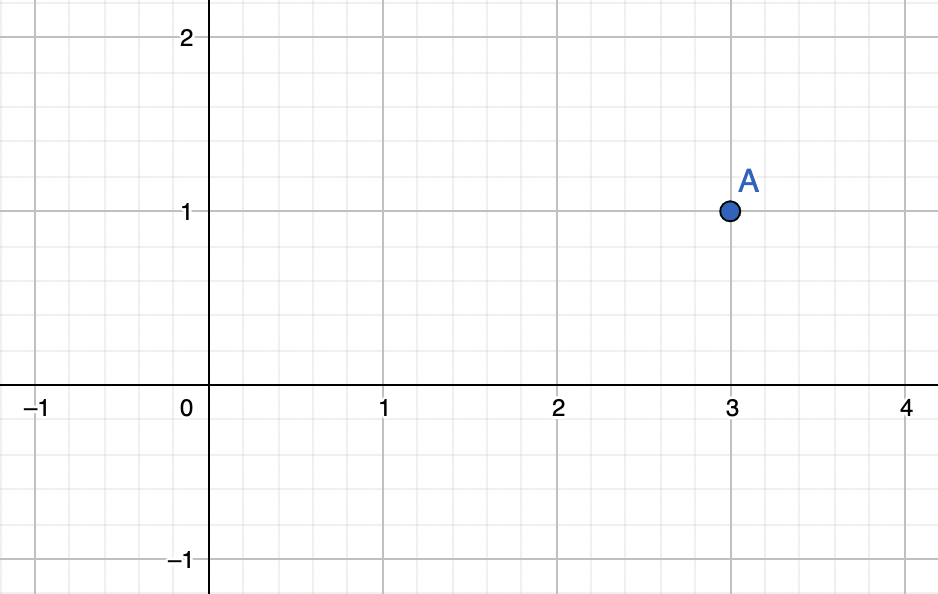
\includegraphics[width=\textwidth]{img/1.png}

\newpage
\subsubsection{Avståndsformeln}

Avståndet mellan två punkter i koordinatsystemet från \ref{Koordinatsystem} kan beräknas med hjälp av Pythagoras Sats från \ref{Pythagoras Sats}. Om vi börjar med två koordinater, $A=(2,2)$ och $B=(4,3)$

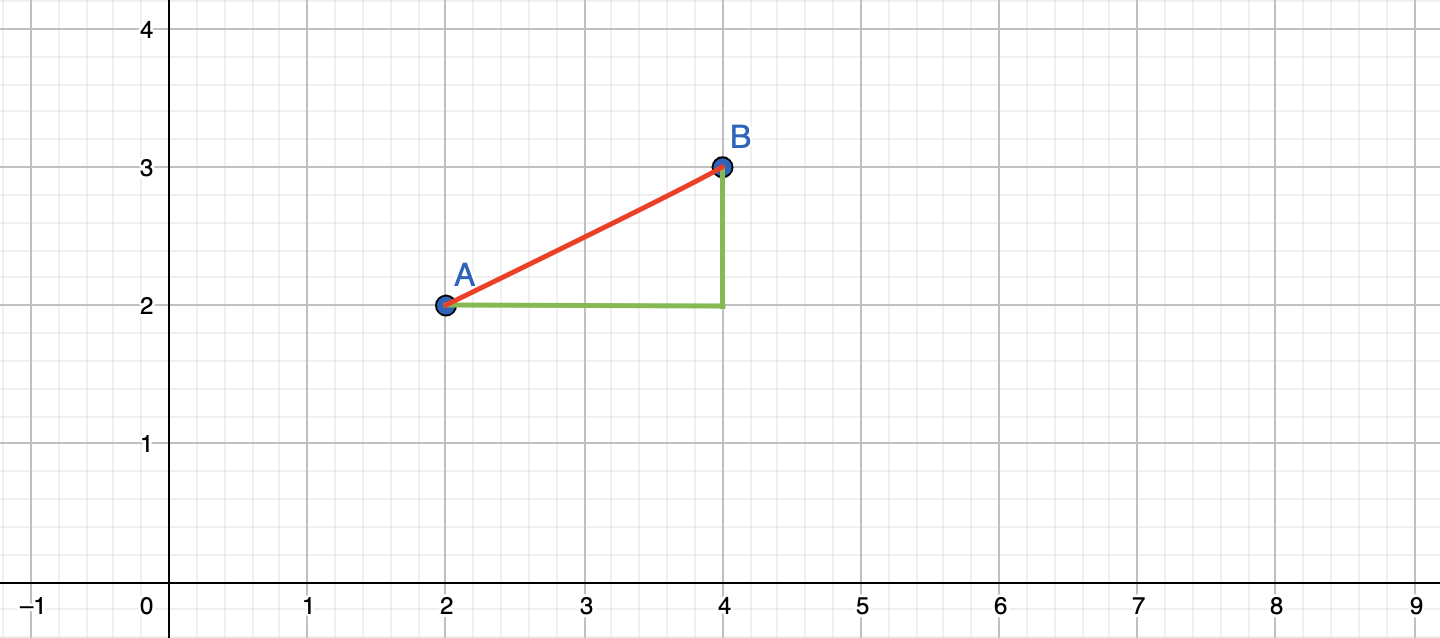
\includegraphics[width=\textwidth]{img/3.png}

Så kan vi se att de bildar en rätvinklig triangel, där en av kateterna är längs x-axeln och den andra längs y-axeln. Avståndet är då den röda linjen. Om vi vet längden av de två kateterna, så kan vi veta längden för hypotenusan, med pythagoras sats.

Längden av kateten längs x-axeln, som vi kan kalla $a$, är då absolutvärdet\footnote{absolutvärdet är distansen från $0$ på tallinjen, så t.ex är |-5| = 5. I fallet ovan så använder vi absolutvärdet då en distans aldrig kan vara negativ, men en differens mellan delar av två koordinater kan det.} av differensen mellan koordinaternas x-värden, så den kateten är

\begin{align}
	a = \\
	|2-4| = \\
	|-2| = \\
	2 \text{ (l.e)}
\end{align}

Vi kan göra exakt samma sak för kateten längs y-axeln, som vi kan kalla för $b$.

\begin{align}
	b = \\
	|2-3| = \\
	|-1| = \\
	1 \text{ (l.e)}
\end{align}

Då vi vill veta längden av hypotenusan, vilket är avståndet mellan koordinaterna, så kan vi lösa ut variabeln $c$ ur pythagoras sats, och sedan sätta in de värden vi har tagit fram.

\begin{align}
	a^2+b^2=c^2 \\
	c = \sqrt{a^2+b^2} \\
	c = \sqrt{2^2+1^2} \\
	c = \sqrt{5} \text{ (l.e)}
\end{align}

Vi kan nu generalisera det vi gjorde ovan. 

Låt $A=(a,b)$, $B=(c,d)$ och $l$  avståndet mellan koordinaterna. Då är

\begin{align}
	l = \sqrt{|a-c|^2+|b-d|^2}
\end{align}

och då absolutvärdefunktionen inte behövs, då vi ändå kvadrerar båda termerna, så kan vi förenkla detta till

\begin{align}
	l = \sqrt{(a-c)^2+(b-d)^2}.
\end{align}

\newpage
\subsubsection{Mittpunktsformeln}

Mittpunksformeln är väldigt enkel. Målet är att hitta den punkt som är mitt emellan två koordinater.

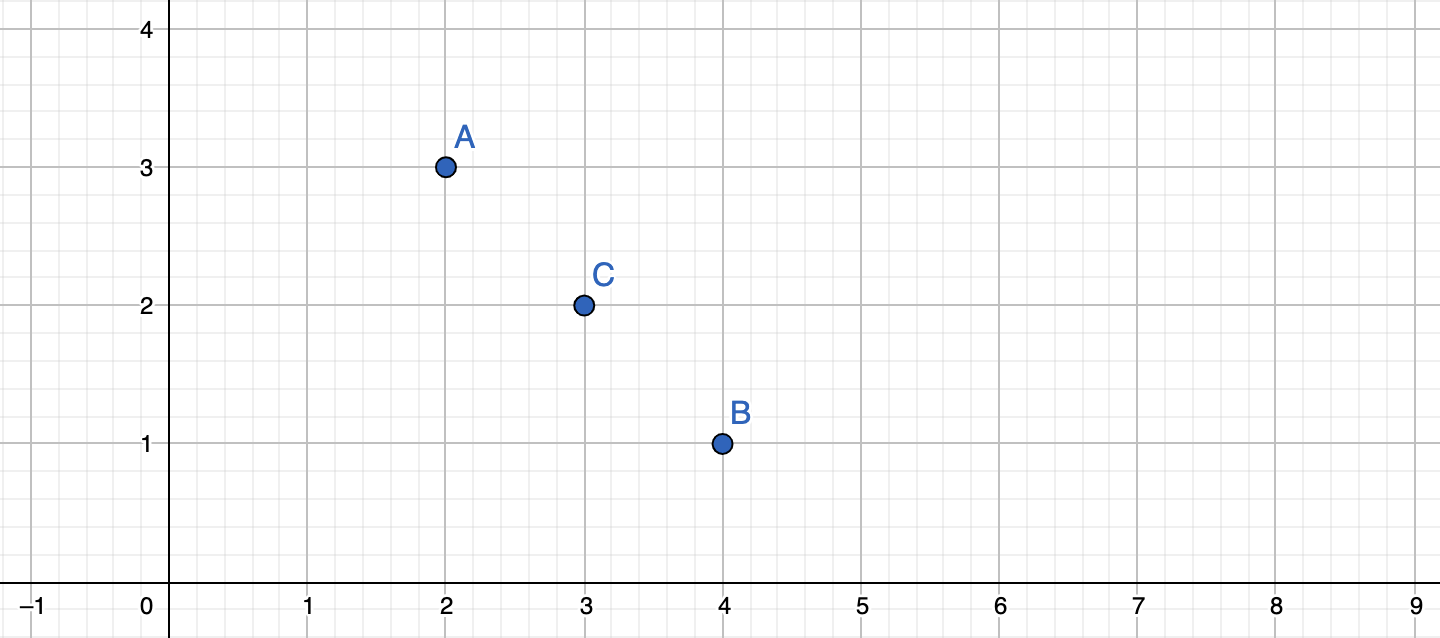
\includegraphics[width=\textwidth]{img/4.png}

Låt $A=(a,b)$, $B=(c,d)$ och låt $C$ vara deras mittpunkt. För att hitta värdet på $C$ så kan vi ta snittvärdet för $x$-värdet och sedan $y$-värdet för $A$ och $B$, vilket är $x$ och $y$-värdet för $C$, då $C$ är mitt emellan. Detta leder till att

\begin{align}
	C = \left(\frac{a+c}{2}, \frac{b+d}{2}\right)
\end{align}

\newpage
\subsection{Funktion}

En funktion inom Matematik 2B är något som översätter ett nummer till ett annat. Ett exempel är denna funktion $f$,

\begin{align}
	f(x) = \frac{1}{2}x-1
\end{align}

som översätter $2$ till $0$, eller $4$ till $1$.

vi kan rita up $f$ grafiskt i koordinatsystemet från \ref{Koordinatsystem}, genom att låta $f(x) = y$.

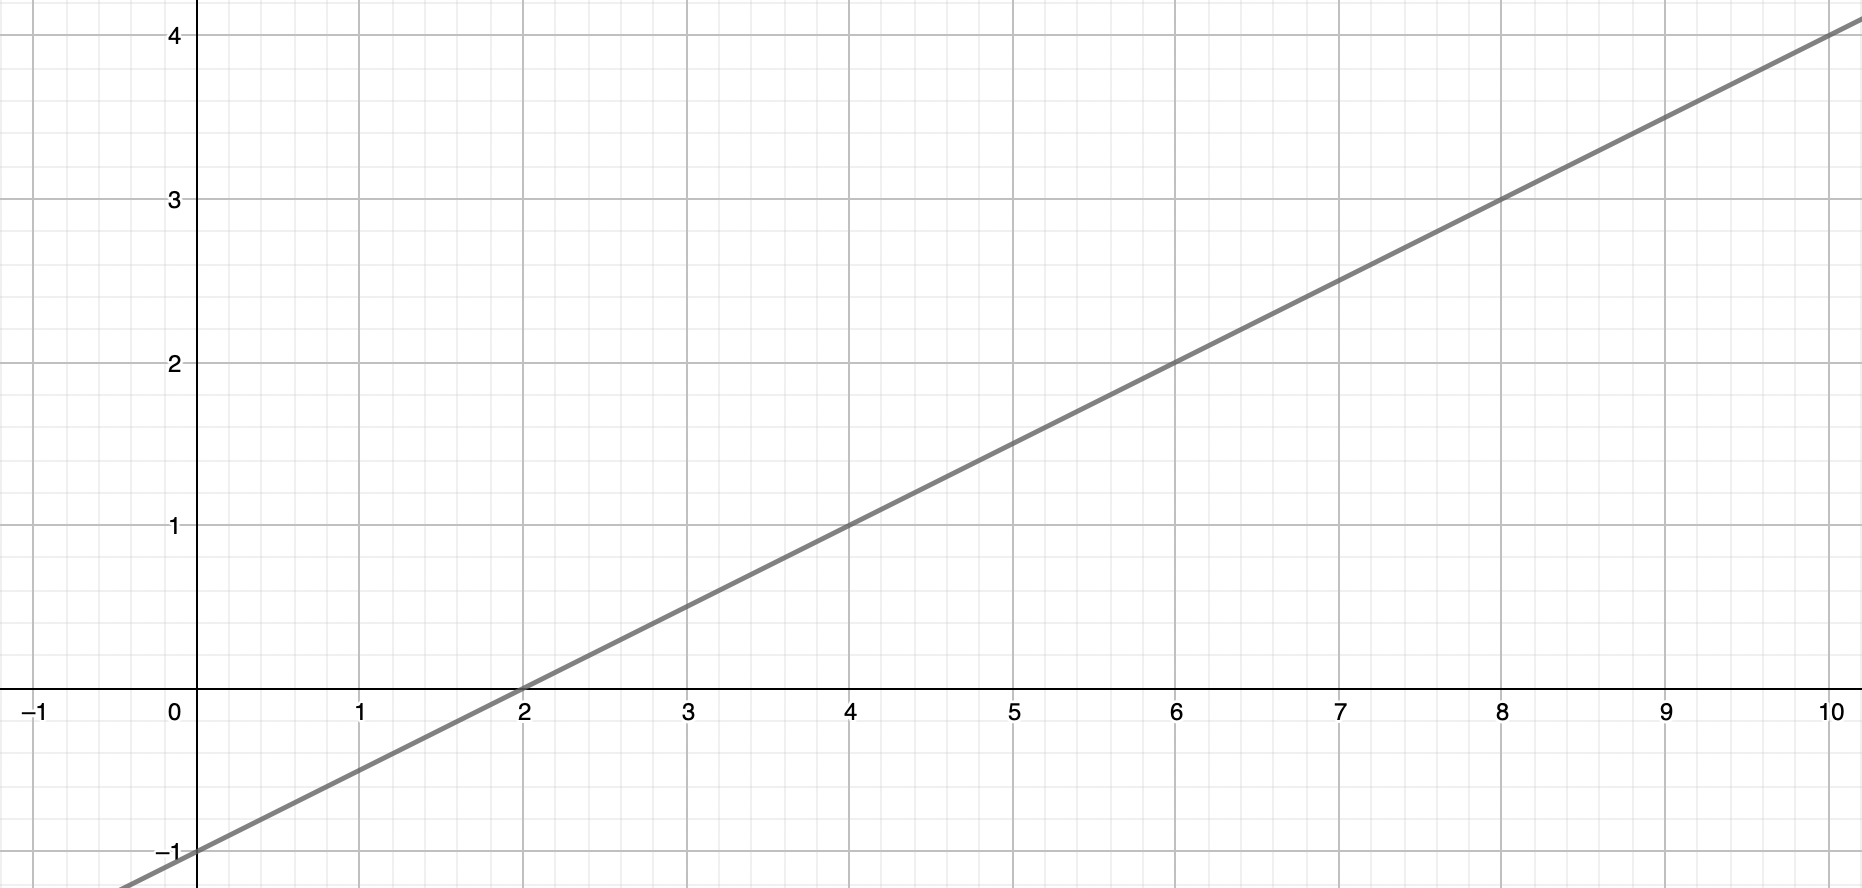
\includegraphics[width=\textwidth]{img/2.png}

\newpage
\subsection{Räta linjens ekvation}

Räta linjens ekvation brukar skrivas såhär:

\begin{align}
	y=kx+m
\end{align}

eller som en funktion:

\begin{align}
	f(x)=kx+m.
\end{align}

$k$-värdet styr förändringshastigheten, alltså hur mycket $y$-värdet förändras av en ändring hos $x$, $\frac{\Delta y}{\Delta x}$. Om $y = 3x$ så kommer $y$-värdet öka med $3$ då $x$-värdet ökar med 1. Om vi väljer två koordinater som ligger på grafen av en linjär funktion $f$, $A=(x_1,y_1)$ och $B=(x_2,y_2)$, så gäller det att

\begin{align}
	k = \frac{\Delta y}{\Delta x} = \frac{y_1-y_2}{x_1-x_2}
\end{align}

$m$-värdet styr hur mycket vi puttar upp eller puttar ner hela grafen, då det bara är en adderad konstant. $m$ värdet är också det $y$-värde där en funktion $f(x)=kx+m$ korsar $y$-axeln, då $f(0)=m$.

\begin{align}
	f(x) = kx+m \Rightarrow f(0) = m
\end{align}

\subsection{Ekvationssystem}

Detta under kallas för ett ekvationssystem. De kan egentligen bestå av flera hundra eller mer ekvationer och variabler, men vi nöjer oss med två.

\begin{align}
	\label{59}
	\begin{cases}
		y+2x=8 \\
		2y-x = 1
	\end{cases}
\end{align}

I ett ekvationssystem så kan tre fall inträffa. 

\begin{itemize}
	\item Ekvationssystemet har en lösning
	\item Ekvationssystemet saknar lösning
	\item Ekvationssystemet har ett oändligt antal lösningar
\end{itemize}

Ett sätt att visualisera dessa tre fall, är att skriva om ekvationerna i ekvationssystemet till formen $y=kx+m$ och sedan tänka på dem som linjer i ett koordinatsystem.

\begin{align}
	\begin{cases}
		y+2x=8 \\
		2y-x = 1
	\end{cases} \Rightarrow 
	\begin{cases}
		y=-2x+8 \\
		y = \frac{1}{2}x+\frac{1}{2}
	\end{cases}
\end{align}

Om två linjer har olika lutning, alltså olika $k$-värde, så kommer linjerna att korsa varann någonstans och därmed ha en lösning (koordinaten av korsningspunkten är lösningen). Om linjerna har samma $k$-värde och olika $m$-värde så är de pararella och möts aldrig, så ekvationssystemet saknar lösning. Om linjerna har samma $k$-värde och samma $m$-värde så möts linjerna på ett oändligt antal koordinater, och därmed har ekvationssystemet ett oändligt antal lösningar. 

Testa att checka vad för fall som gäller för ekvationsystemet i \eqref{59}!

\subsubsection{Substitutionsmetoden}
\label{Substitutionsmetoden}

Substitutionsmetoden är en metod för att få fram lösningen på ett ekvationsystem. Här under har vi ett ekvationsysstem med två variabler

\begin{align}
	\begin{cases}
		y+2x=8 \\
		2y-x = 1
	\end{cases}
\end{align}

För att lösa det, så kan vi följa en viss stegmetod

\begin{enumerate}
	\item Lös ut en variabel ur den ena ekvationen.
	\item Ersätt variabeln i den andra ekvationen med detta uttryck och lös ekvationen.
	\item Lösningen till ekvationen sätts in i någon av de ursprungliga ekvationerna, som därefter löses.
\end{enumerate}

I fallet ovan så kan det se ut såhär:

Steg 1, vi börjar med att lösa ut en variabel ur den ena ekvationen.
\begin{align}
	y+2x = 8 \Rightarrow y = 8-2x \\
\end{align}

Steg 2, vi ersätter variabeln i den andra ekvationen med detta uttryck, så att det bara finns en variabel i ekvationen, och löser den.
\begin{align}
	2y-x = 1 \\
	2(8-2x)-x = 1 \\
	16-4x-x = 1 \\
	16-5x = 1 \\
	5x + 1 = 16 \\
	5x = 15 \\
	x = 3
\end{align}

Steg 3, vi sätter in lösningen till den andra ekvationen i den ursprungliga ekvationen, och därefter löser den med.

\begin{align}
	y+2x = 8 \\
	y+2(3) = 8 \\
	y+6 = 8 \\
	y = 2
\end{align}

Därmed är lösningen på ekvationssystemet

\begin{align*}
	\begin{cases}
		x = 3 \\
		y = 2
	\end{cases}
\end{align*}

\newpage
\subsubsection{Additionsmetoden}

Additionsmetoden fungerar lite annorlunda, men denna är min personliga preferens i de flesta fallen. Istället för att lösa ut en variabel och sätta in den i en annan ekvation så multiplicerar vi hela ekvationer med konstanter och adderar in dem i andra för att eliminera variabler. Så här går det till, med samma exempel som i \ref{Substitutionsmetoden}:

\begin{align}
	\begin{cases}
		y+2x=8 \\
		2y-x = 1
	\end{cases}
\end{align}

Målet är att eliminera en variabel i varje ekvation så att vi får ekvationer med ensamma variabler i, vilket då är enkelt att lösa. Vi börjar med att multiplicera rad 1 med konstanten $(-2)$.

\begin{align}
	\begin{cases}
		-2y-4x=-16 \\
		2y-x = 1
	\end{cases}
\end{align}

Därefter kan vi addera rad 1 till rad 2

\begin{align}
	\begin{cases}
		-2y-4x=-16 \\
		-5x = -15
	\end{cases}
\end{align}

och förenkla rad 2 genom att dividera båda sidor med $(-5)$.

\begin{align}
	\begin{cases}
		-2y-4x=-16 \\
		x = 3
	\end{cases}
\end{align}

Därefter kan vi addera in rad 2, multiplicerat med konstanten $4$, i rad 1 för att eliminera $x$-variabeln där.

\begin{align}
	\begin{cases}
		-2y=-4 \\
		x = 3
	\end{cases}
\end{align}

Sedan kan vi förenkla rad 1 genom att dividera med $(-2)$ på båda sidor

\begin{align}
	\begin{cases}
		y=2 \\
		x = 3
	\end{cases}
\end{align}

Därmed har vi samma svar som i \ref{Substitutionsmetoden}, men genom en annan metod.








































\section{Ickelinjära ekvationer och funktioner}
\subsection{Konjugat och kvadreringsreglerna}

Detta är bara att memorera. \bigskip

\begin{theorem}{Konjugatregeln}
	\begin{align}
	(a+b)(a-b) = a^2-b^2
	\end{align}
\end{theorem}

Motivering:

\begin{align}
	(a+b)(a-b) = \\ 
	a^2 - ab + ab + b^2 = \\
	a^2 + b^2
\end{align}

\begin{theorem}{Kvadreringsreglerna}
	\begin{align}
		(a+b)^2 = a^2+2ab+b^2 \\
		(a-b)^2 = a^2-2ab+b^2
	\end{align}
\end{theorem}

Motivering för första:

\begin{align}
	(a+b)^2 = \\
	(a+b)(a+b) = \\
	a^2 + ab + ba + b^2 = \\
	a^2 + 2ab + b^2
\end{align}

Motivering för andra:

\begin{align}
	(a-b)^2 = \\
	(a-b)(a-b) = \\
	a^2 - ab - ba + (-b)^2 = \\
	a^2 - 2ab + b^2
\end{align}

\newpage
\subsection{Polynom}

\begin{definition}
	En polynom är en funktion som kan skrivas i formen
	
	\begin{align}
		f(x) = a_0x^0 + a_1x^1 + a_2x^2 + \hdots + a_nx^n
	\end{align}
	
	där $n$ är ett positivt heltal från $0$ och uppåt och $a_0, a_1, a_2, \hdots, a_n$ är konstanter.
\end{definition}

Utifrån detta så kan vi se att linjära funktioner är polynomer där konstanten med index 1 inte är lika med noll, men att alla konstanter med högre index är lika med noll. Något som Matematik 2B kör hårt på är dock just andragradsfunktioner, vilket är polynomer där konstanten med index 2 inte är lika med noll men alla konstanter med högre index är lika med noll.

En andragradsfunktion kan därmed skrivas i formen

\begin{align}
	f(x) = ax^2 + bx + c
\end{align}

som det görs i de allra flesta matteböcker.










































































\section{Statistik}
\subsection{Konjugat och kvadreringsreglerna}

Detta är bara att memorera. \bigskip

\begin{theorem}{Konjugatregeln}
	\begin{align}
	(a+b)(a-b) = a^2-b^2
	\end{align}
\end{theorem}

Motivering:

\begin{align}
	(a+b)(a-b) = \\ 
	a^2 - ab + ab + b^2 = \\
	a^2 + b^2
\end{align}

\begin{theorem}{Kvadreringsreglerna}
	\begin{align}
		(a+b)^2 = a^2+2ab+b^2 \\
		(a-b)^2 = a^2-2ab+b^2
	\end{align}
\end{theorem}

Motivering för första:

\begin{align}
	(a+b)^2 = \\
	(a+b)(a+b) = \\
	a^2 + ab + ba + b^2 = \\
	a^2 + 2ab + b^2
\end{align}

Motivering för andra:

\begin{align}
	(a-b)^2 = \\
	(a-b)(a-b) = \\
	a^2 - ab - ba + (-b)^2 = \\
	a^2 - 2ab + b^2
\end{align}

\newpage
\subsection{Polynom}

\begin{definition}
	En polynom är en funktion som kan skrivas i formen
	
	\begin{align}
		f(x) = a_0x^0 + a_1x^1 + a_2x^2 + \hdots + a_nx^n
	\end{align}
	
	där $n$ är ett positivt heltal från $0$ och uppåt och $a_0, a_1, a_2, \hdots, a_n$ är konstanter.
\end{definition}

Utifrån detta så kan vi se att linjära funktioner är polynomer där konstanten med index 1 inte är lika med noll, men att alla konstanter med högre index är lika med noll. Något som Matematik 2B kör hårt på är dock just andragradsfunktioner, vilket är polynomer där konstanten med index 2 inte är lika med noll men alla konstanter med högre index är lika med noll.

En andragradsfunktion kan därmed skrivas i formen

\begin{align}
	f(x) = ax^2 + bx + c
\end{align}

som det görs i de allra flesta matteböcker.










































































\end{document}